\documentclass[12pt]{article}
\usepackage{hyperref}
\usepackage{graphicx}
\usepackage{mathtools}
\usepackage[margin=1in, paperwidth=8.5in, paperheight=11in]{geometry}
\begin{document}
\title{Istanbul Technical University- Spring 2017 \\ BLG527E Machine Learning \\ Homework 2}
\author{Omid Abdollahi Aghdam \\
student number: 504151520\\
\href{mailto:abdollahi15@itu.edu.tr}{abdollahi15@itu.edu.tr}\\
\href{mailto:abdollahi.omid@gmail.com}{abdollahi.omid@gmail.com}
}
\date{\today}
\maketitle
\newpage

\textbf{Note:} Running \textit{discriminant.py} will save confusion matrix figures in the same directory and write the asked questions in \textit{Q1)} into \textit{output.txt} file.

\textbf{Q1)}\\*
\textbf{Q1a)} Equation \ref{naive} is implemented to calculate the discriminant function.  
\begin{equation}\label{naive}
	g_{i}(x) = -\frac{1}{2}\Sigma_{j=1}^{d} (\frac{x_{j}^{t} - m_{ij}}{s_{j}})^{2} + log\hat{P}(C_{i})
\end{equation}

\textbf{Q1b)} In this question also, quation \ref{navie} is implemented to calculate the discriminant function. However, as we assume that all variance are equal formula simplified to equation \ref{mean}   

\begin{equation}\label{mean}
	g_{i}(x) = -\frac{1}{2s^{2}}\Sigma_{j=1}^{d} (x_{j}^{t} - m_{ij})^{2} + log\hat{P}(C_{i})	
\end{equation}

Class distribution are shown in Figure \ref{fig:dist}.
\begin{figure}[ht]
	\centerline{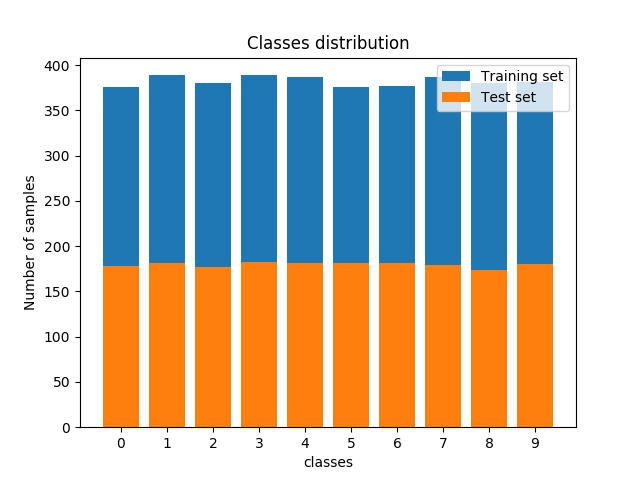
\includegraphics[width=3in]{dist.png}}
	\caption{Class distribution in the train and test dataset.}
	\label{fig:dist}
\end{figure}

\textbf{Q1c)} Assuming that all variances are equal (Q1b) has the best test error.\\*
\begin{center}
		Test error of Q1a: 0.106845\\* 
		Test error of Q1b: 0.106288	\\
\end{center}
\textbf{Test error per class when assuming diagonal common covariance matrix:}
\begin{center}
	Class 0 error: 0.005618\\* 
	Class 1 error: 0.258242\\* 
	Class 2 error: 0.118644\\* 
	Class 3 error: 0.136612\\* 
	Class 4 error: 0.060773\\* 
	Class 5 error: 0.054945\\* 
	Class 6 error: 0.038674\\* 
	Class 7 error: 0.033520\\* 
	Class 8 error: 0.212644\\* 
	Class 9 error: 0.150000 
\end{center}
\textbf{Test error per class when assuming all variance are equal:}
\begin{center}
Class 0 error: 0.016854 \\*
Class 1 error: 0.252747 \\*
Class 2 error: 0.112994 \\*
Class 3 error: 0.114754 \\*
Class 4 error: 0.088398 \\*
Class 5 error: 0.060440 \\*
Class 6 error: 0.033149 \\*
Class 7 error: 0.050279 \\*
Class 8 error: 0.206897 \\*
Class 9 error: 0.127778 
\end{center}
Figures \ref{fig:traindiag} and \ref{fig:testdiag} show confusion matrix for train set and test when we assume a diagonal common covariance matrix. Also, Figures \ref{fig:traineq} and \ref{fig:testeq} show confusion matrix when we assume all variance are equal.\\
\begin{figure}[ht]
  \centerline{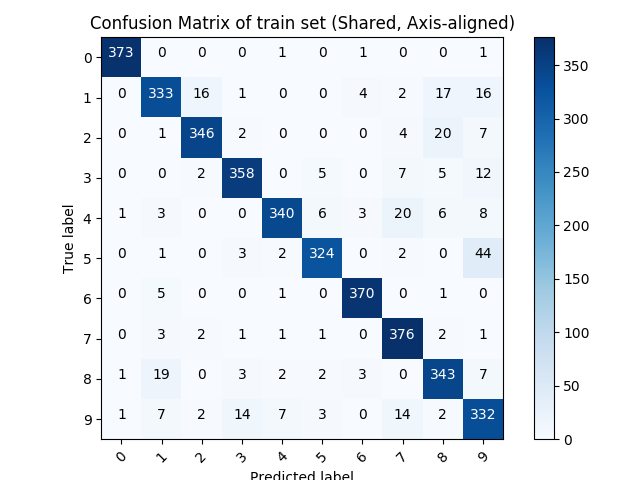
\includegraphics[width=2.5in]{traindiag.png}}
  \caption{Confusion Matrix of training set Q1a.}
  \label{fig:traindiag}
\end{figure}
\begin{figure}[ht]
	\centerline{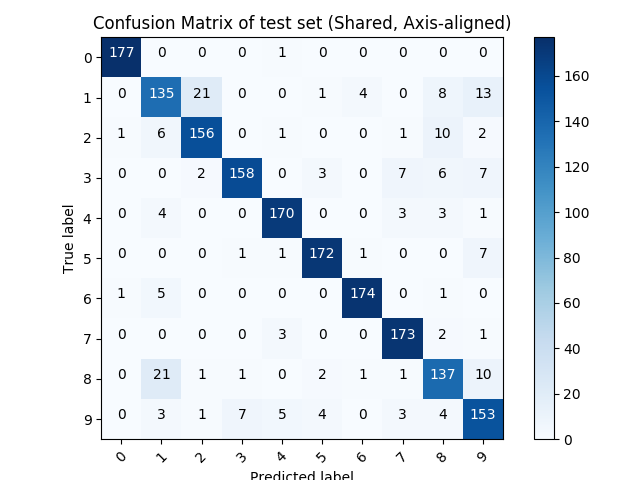
\includegraphics[width=2.5in]{testdiag.png}}
	\caption{Confusion Matrix of test set Q1a.}
	\label{fig:testdiag}
\end{figure}
\begin{figure}[ht]
	\centerline{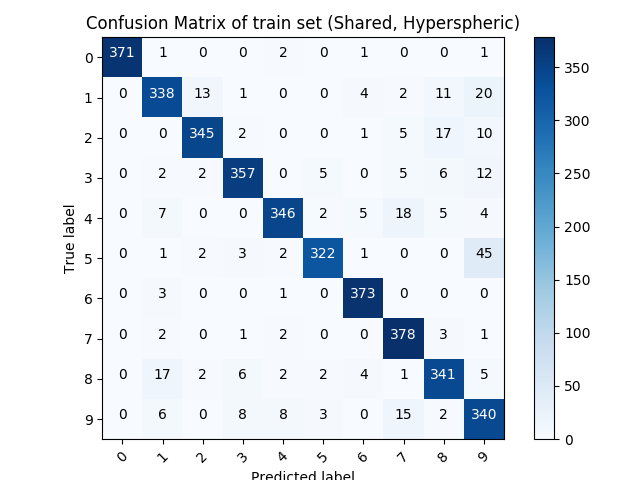
\includegraphics[width=2.5in]{traineq.png}}
	\caption{Confusion Matrix of training set Q1b.}
	\label{fig:traineq}
\end{figure}
\begin{figure}[ht]
	\centerline{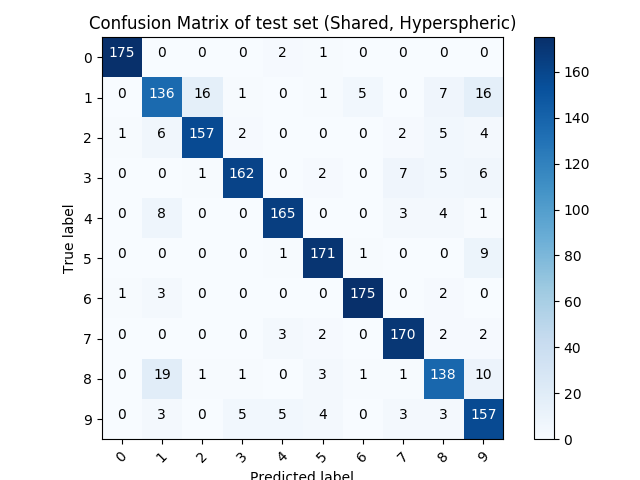
\includegraphics[width=2.5in]{testeq.png}}
	\caption{Confusion Matrix of test set Q1b.}
	\label{fig:testeq}
\end{figure}
As it can be seen in test set confusion matrix in both assumption, mostly, class 1 is miss-predicted as classes 2, 8 or 9, and class 8 is misclassified as 1 or 9.\\
\newpage
\newpage
\textbf{Q2):} Running \textit{lda.py} will plot and save Figures \ref{fig:trainopt} and \ref{fig:testopt} in the same directory.
\begin{figure}[ht]
	\centerline{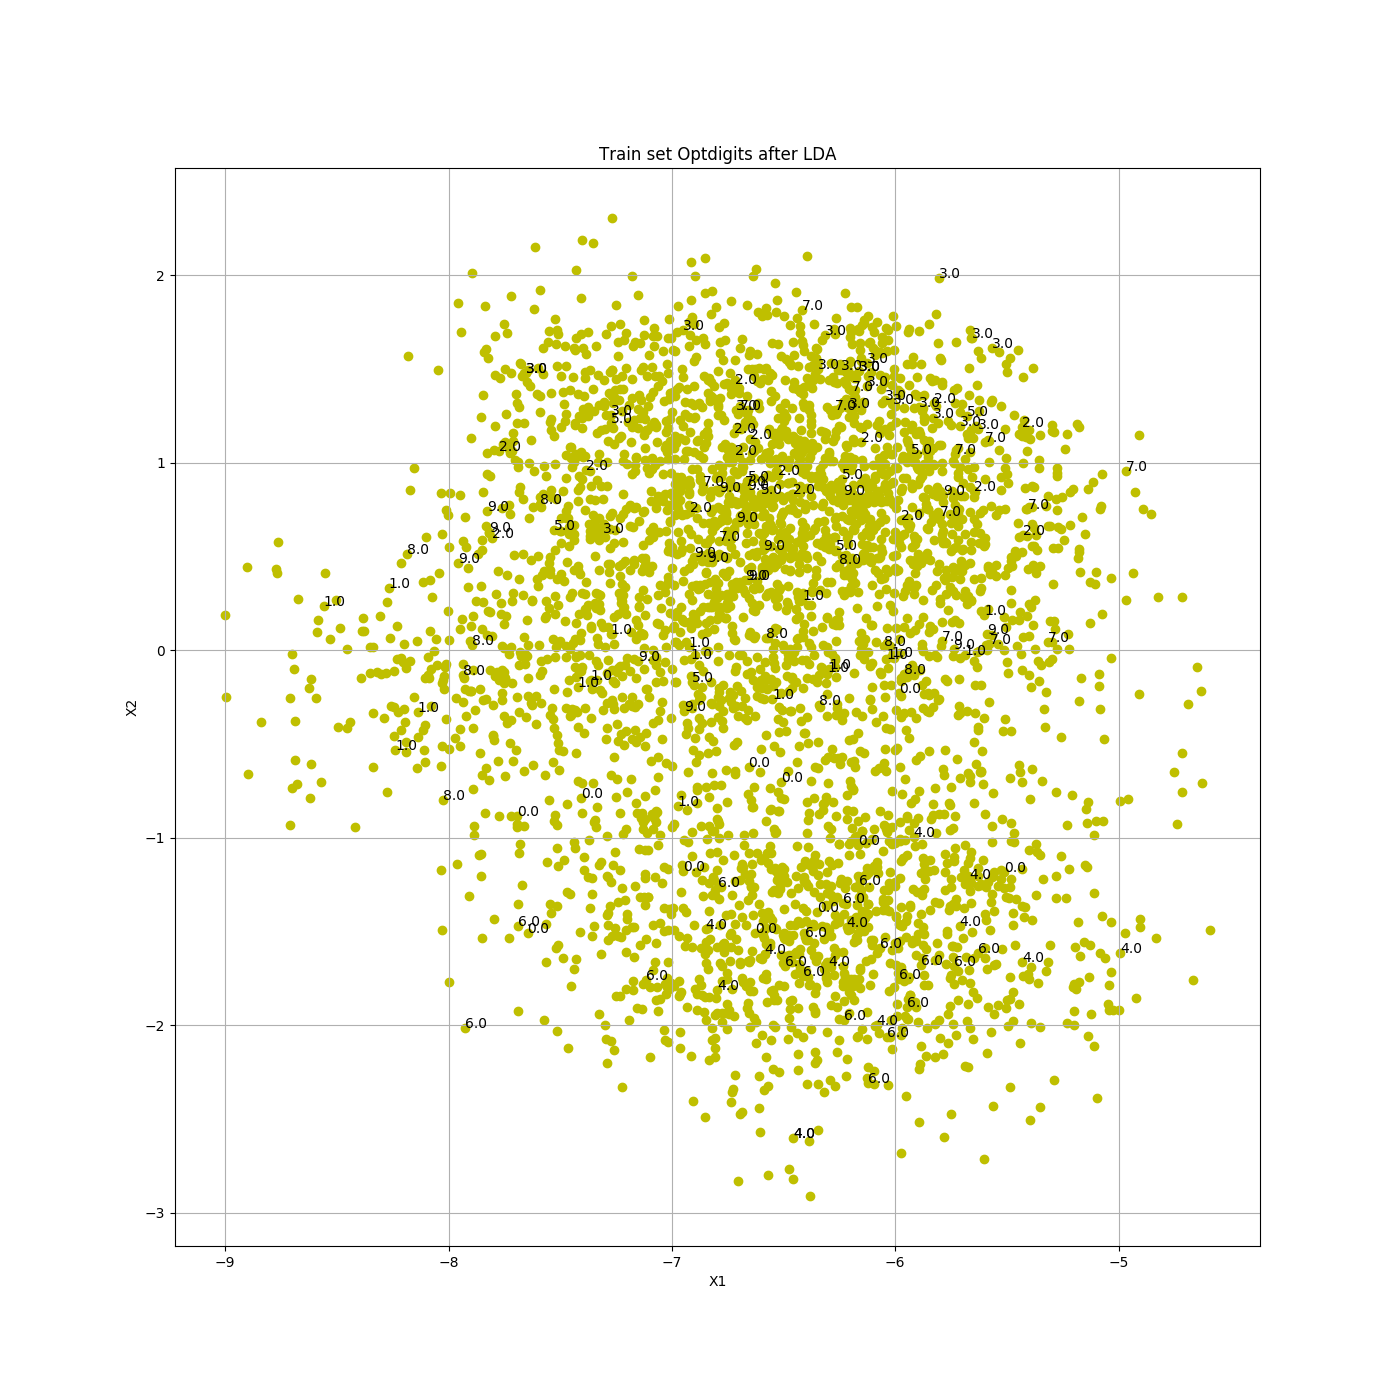
\includegraphics[width=5in]{trainoptdigits.png}}
	\caption{Visualizing train dataset after projecting to 2d using LDA.}
	\label{fig:trainopt}
\end{figure}
\begin{figure}[ht]
	\centerline{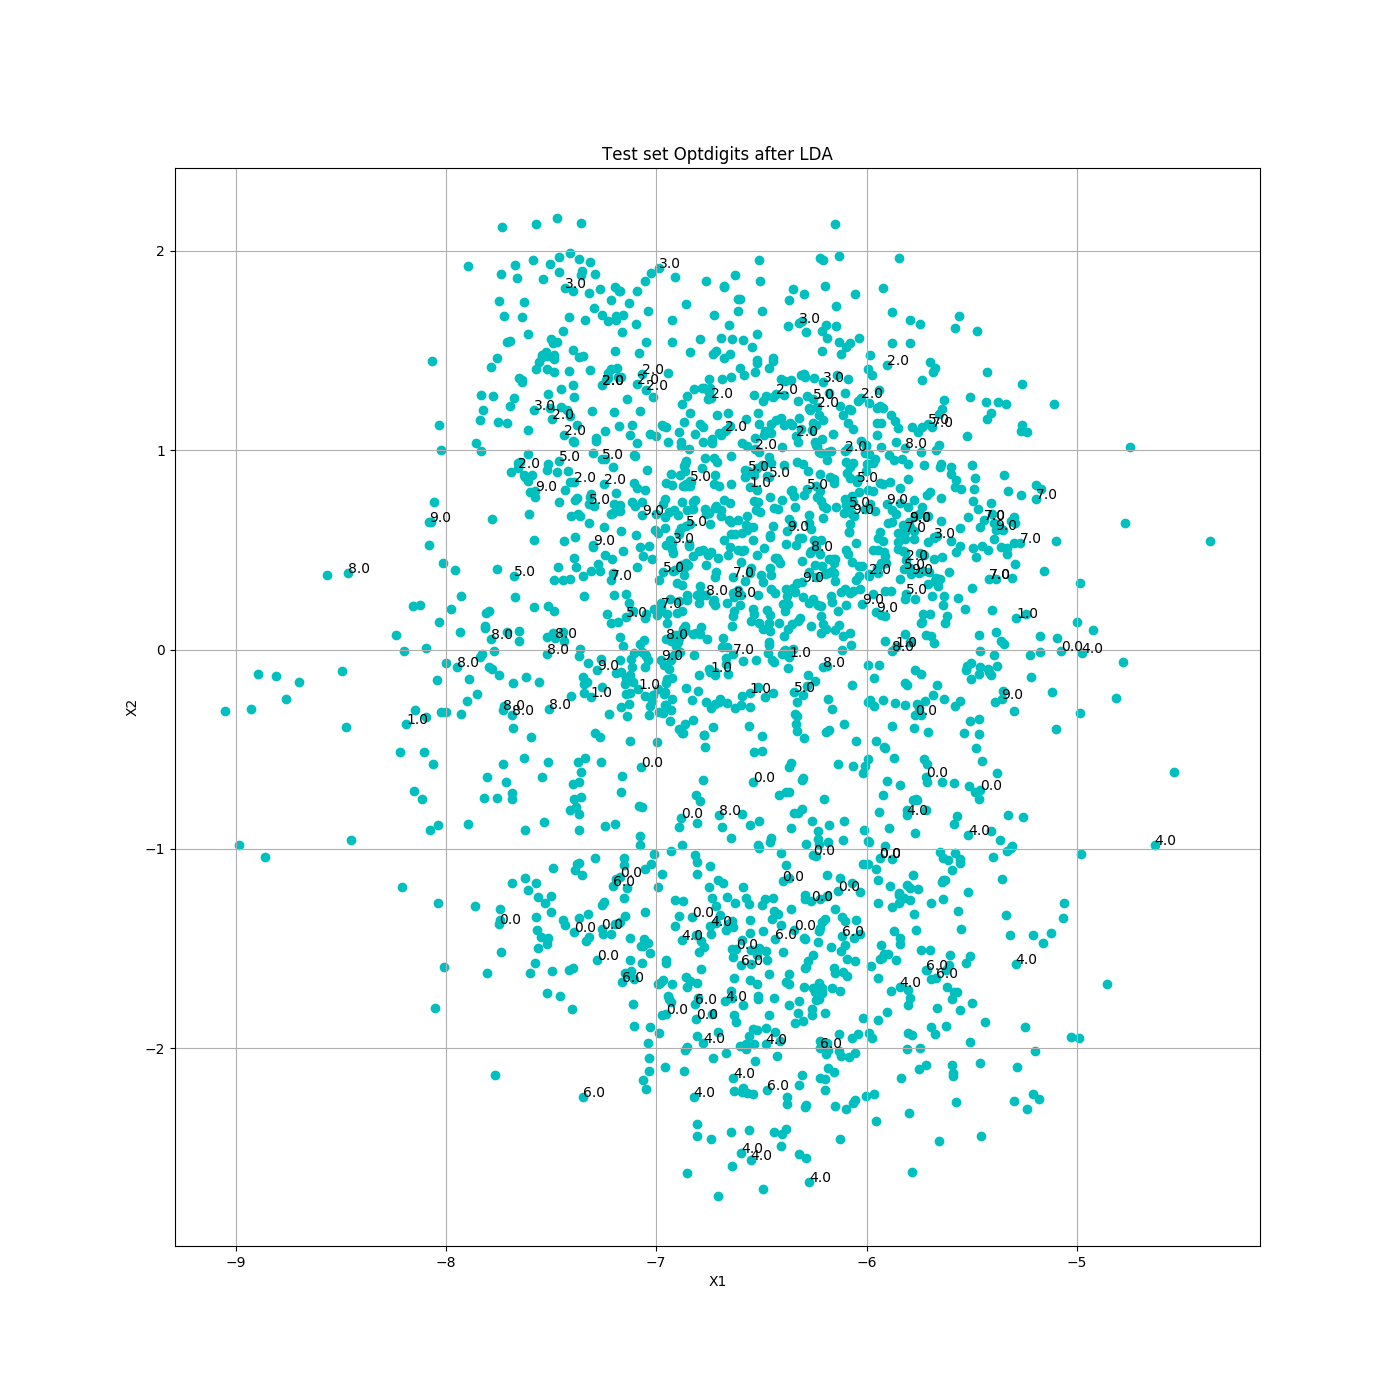
\includegraphics[width=5in]{testoptdigits.png}}
	\caption{Visualizing test dataset after projecting to 2d using LDA.}
	\label{fig:testopt}
\end{figure}
\end{document}